\section{Introduction}\label{sec:intro}

LLM agents are increasingly allowed to call APIs, read databases and take actions with real consequences, such as issuing refunds or deleting resources. Agents treat tool outputs as evidence about the outside world. The most dangerous failure is a \emph{silent tool failure}: the call succeeds and the output is schema-valid, but its content is wrong or stale.

A natural defence is \emph{cross-verification}: before acting, the agent consults a second tool (a \emph{corroborator}) and proceeds only if the two agree. The number of tools, however, is not the number of independent sources of evidence. Two differently named tools may call the same provider. When that provider is wrong, both tools are wrong in the same way, and the agent sees false agreement (\cref{fig:problem}). This is the familiar \emph{common-mode failure} of dependable systems~\cite{kl86}, and correlated errors have also been observed across LLMs~\cite{ce25}.

\begin{figure}[t]
  \centering
  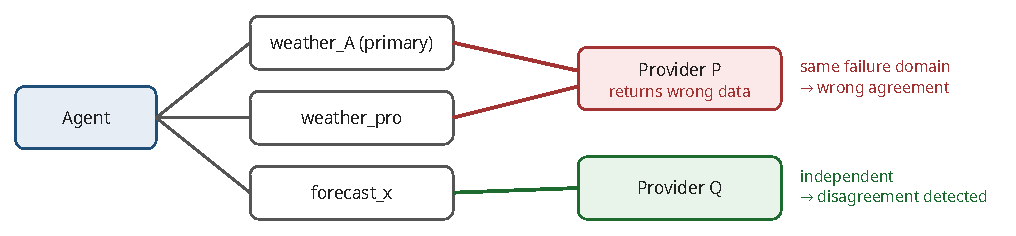
\includegraphics[width=0.85\linewidth]{figures/problem-common-mode.pdf}
  \caption{The primary \code{weather\_A} and \code{weather\_pro} have different names but call the same Provider~P, so they share a failure domain. When P returns wrong data, choosing \code{weather\_pro} as corroborator yields false agreement; \code{forecast\_x} calls an independent Provider~Q and exposes the disagreement. Illustrative example.}
  \label{fig:problem}
\end{figure}

If the agent knows which tool belongs to which failure domain, it can choose an independent corroborator. VP-Control~\cite{vpc26} measured this with a strong design (preregistration, a live study): under a common-stale regime, false approval is 91.5\% when both verifier calls share the source and 9.8\% when one uses an independent source. EFD~\cite{efd26} proves that adding reviewers cannot repair a shared upstream. Both \emph{assume that lineage labels are available and correct}. Bara~\cite{bara26} shows why this assumption matters: from report content alone one cannot distinguish independent reports from copies of the same evidence, so information about sources must come from outside. In practice that information comes from tool names, descriptions and documentation, and it can be missing or wrong. Three questions follow, and they are the subject of this paper.

\paragraph{Research questions.}
\begin{itemize}
  \item \textbf{RQ1 (label quality).} \emph{Under class-conditional failure-domain label errors, for which combinations of shared-dependency recall $r$ and false-sharing rate $\varphi$ does failure-domain-aware selection beat, match, or lose to random selection?}
  \item \textbf{RQ2 (real metadata).} \emph{Among open-source MCP servers that provide the same information type, how often do two servers share an upstream data provider, and how well does agent-visible metadata reveal that sharing?}
  \item \textbf{RQ3 (LLM behaviour).} \emph{When an LLM agent must choose a corroborating tool from real MCP tool descriptions, does adding the upstream provider to the descriptions reduce how often it chooses a corroborator that shares the primary's provider?}
\end{itemize}
A \emph{baseline experiment} (\cref{sec:baseline}) precedes them. It asks what independent corroboration achieves when metadata is accurate, replicating VP-Control in another domain; it is not a new finding and not a main research question.

\paragraph{Findings in brief.} (i)~A single quantity, $J=r-\varphi$, decides whether label-guided selection helps, does nothing or harms; we prove this and confirm it in a preregistered simulation. (ii)~Real MCP metadata rarely names the provider, but mostly names it correctly when it does. (iii)~LLMs act on provider labels, but how depends on the prompt: with a request for independence a label cuts shared choices sharply, with a neutral request it raises them.

\paragraph{Contributions.} (1)~A simple condition, with a proof, that tells when failure-domain metadata helps, does nothing or harms, together with a preregistered test. (2)~Empirical evidence, replicated on two samples, on the quality of real MCP server metadata, including predictions that failed. (3)~A first measurement of how LLMs choose a corroborator from real tool descriptions, with a causal label-inversion test and a reversal under a neutral prompt. (4)~A controlled replication of the baseline with a negative robustness result and a power analysis. We propose no new algorithm and claim no superiority over prior work.

\paragraph{Chronology.} RQ1, RQ2 and RQ3 were formulated \emph{after} the baseline results were known and after we found VP-Control; RQ3 was posed after the survey results. Every subsequent data collection and test followed a protocol written and confirmed in advance, and every later change was logged as a dated amendment. These protocols are internal, not registered with an independent registry. In this paper, ``the first author'' is Lương Tuấn Kiệt, who designed and ran the study; the other authors are members of the same course group.

\paragraph{Roadmap.} \Cref{sec:formulation} fixes the formulation, \cref{sec:related} reviews related work, and \cref{sec:baseline} reports the baseline. \Cref{sec:rq1,sec:rq2,sec:rq3} address the three research questions, \cref{sec:discussion} discusses implications, \cref{sec:threats} lists threats to validity and \cref{sec:conclusion} concludes.
